% 第四章 系统总体设计

\chapter{系统总体设计}


\section{系统总体架构}

FreeFlow采用桌面端、Web2.5后端、智能合约和IPFS存储协同的架构。桌面端负责用户交互、音频播放、本地缓存和钱包交互；后端负责SIWE认证、Pinata上传代理、发行数据管理、资源检索、购买记录和评论；智能合约负责链上发布、访问凭证、购买授权和收益分账；IPFS/Pinata负责保存音频、封面和metadata资源。整体设计遵循“低频且需要强可信的数据上链，高频且需要快速查询的数据链下处理”的原则：作品发布结果、访问授权和交易记录放在链上，评论、搜索索引、登录会话和上传状态等高频数据放在链下。

系统总体架构如图\ref{fig:system_architecture}所示。Electron桌面端通过Web2.5 API访问后端业务服务，通过ethers.js与Sepolia测试网合约交互，并通过本地音频代理播放IPFS gateway音频资源。后端通过Prisma维护PostgreSQL中的用户、发行、存储、购买和评论数据，同时代理Pinata上传，形成链上状态和链下索引协同的系统结构。之所以不把评论、全文检索索引和会话信息直接写入链上，是因为这类数据更新频繁、查询维度多、需要分页与条件过滤，若全部转化为链上写入和链上读取，不仅会持续消耗gas，还会受到区块确认延迟与链上检索能力限制，不利于音乐应用中的即时交互与内容服务\cite{Eren2025,Friedl2024}。

\begin{figure}[htbp]
    \centering
    
\includegraphics[width=0.95\textwidth]{figures/out/system_architecture.png}
    \caption{FreeFlow系统总体架构图}
    \label{fig:system_architecture}
\end{figure}


\section{功能模块设计}

系统功能模块可划分为用户资料与认证模块、创作者工作台模块、素材上传模块、链上发布模块、资源检索模块、购买与访问验证模块、播放与缓存模块、链上音乐库模块和评论模块。需要说明的是，当前模块划分围绕作品发布、访问控制、资源发现与基础互动展开，不包含治理代币、提案投票或自治审核等治理模块。

\begin{table}[htbp]
    \linespread{1.5}
    \zihao{5}
    \songti
    \centering
    \caption{系统功能模块设计}\label{tab:module_design}
    \begin{tabular}{|l|p{10cm}|}
        \hline
        模块        & 设计说明                                           \\ \hline
        用户资料与认证模块 & 使用SIWE完成钱包登录，并在后端创建用户、钱包身份和会话                  \\ \hline
        创作者工作台模块  & 管理发行草稿、作品信息、发布阶段、素材状态和链上发布结果                   \\ \hline
        素材上传模块    & 经后端将音频、封面和metadata上传到Pinata，并保存StorageObject   \\ \hline
        链上发布模块    & 调用PlatformHub发布作品，解析事件并回写tokenId、splitter和交易哈希 \\ \hline
        资源检索模块    & 检索已发布链上音乐资源，并基于排序算法返回可解释结果                     \\ \hline
        购买访问模块    & 查询销售配置、调用buyAccess、记录购买交易并验证访问凭证               \\ \hline
        播放缓存模块    & 通过音频代理支持IPFS gateway音频播放、Range请求和本地缓存          \\ \hline
        评论模块      & 支持用户查看和发布作品评论                                  \\ \hline
    \end{tabular}
\end{table}


\section{业务流程设计}

\subsection{创作者发布流程}

创作者发布流程如图\ref{fig:release_workflow}所示。该流程以创作者工作台为入口，依次完成发行草稿维护、素材上传、元数据生成、合约发布和链上索引回写。该流程的关键设计点在于：音频文件、封面文件和扩展metadata由IPFS承载，链上只记录metadata URI、销售配置和访问凭证等关键状态，从而避免把大体积媒体内容直接写入链上。

\begin{figure}[htbp]
    \centering
    
\includegraphics[width=0.98\textwidth]{figures/out/release_workflow.png}
    \caption{创作者链上音乐发布流程图}
    \label{fig:release_workflow}
\end{figure}

创作者发布流程的主要步骤如下：

\begin{enumerate}
    \item 用户连接钱包并完成SIWE登录。
    \item 创作者在工作台创建发行草稿。
    \item 编辑标题、歌手、专辑、流派、描述、访问模式、价格和分账信息。
    \item 选择音频和封面文件，系统读取并校验音频metadata。
    \item 后端代理上传音频和封面到Pinata，并保存CID。
    \item 桌面端生成作品元数据文件，并上传到Pinata。
    \item 桌面端调用PlatformHub合约发布作品。
    \item 系统解析链上事件，将tokenId、splitter地址、交易哈希和区块号回写后端。
\end{enumerate}

\subsection{用户购买播放流程}

用户购买播放流程如图\ref{fig:purchase_playback_sequence}所示。系统先通过后端检索和解析链上资源，再以合约访问状态决定是否需要购买，最后将拥有访问权的作品加入链上音乐库并交由音频代理播放。该流程体现了“链下负责组织资源与加速查询，链上负责判定访问资格”的分工方式：检索与详情展示依赖链下索引，访问权确认依赖链上合约结果。

\begin{figure}[htbp]
    \centering
    
\includegraphics[width=0.95\textwidth]{figures/out/purchase_playback_sequence.png}
    \caption{用户购买与播放流程图}
    \label{fig:purchase_playback_sequence}
\end{figure}

用户购买播放流程的主要步骤如下：

\begin{enumerate}
    \item 用户输入关键词检索链上音乐资源。
    \item 后端召回已发布资源并进行排序。
    \item 用户进入链上音乐详情页。
    \item 桌面端读取链上销售配置和访问状态。
    \item 若作品公开，用户可直接加入链上音乐库并播放。
    \item 若作品付费，用户调用buyAccess购买访问权。
    \item 购买成功后，系统记录购买交易并将作品加入链上音乐库。
    \item 用户通过音频代理播放或下载作品。
\end{enumerate}


\section{数据库设计}

FreeFlow同时使用客户端SQLite数据库和服务器PostgreSQL数据库。客户端数据库以\texttt{database.sqlite}文件形式存放于用户本地数据目录中，主要保存本地音乐库、歌单关系、链上音乐库投影、下载状态和应用启动会话；服务器数据库由Prisma管理，主要保存用户身份、SIWE认证会话、IPFS存储对象、创作者发行项目、购买交易投影和评论数据。两类数据库的职责边界不同：SQLite面向桌面端本地播放体验和离线管理，PostgreSQL面向Web2.5业务协同和链上资源索引。系统采用双数据库设计，是因为播放缓存、会话状态、评论列表和搜索排序都依赖频繁更新、分页查询与多条件过滤，这类数据更适合由本地数据库或关系型数据库承载。

\subsection{客户端SQLite数据库设计}

客户端SQLite数据库采用Sequelize模型定义。其核心ER关系如图\ref{fig:client_sqlite_er}所示。\texttt{track}表保存本地音乐、外部平台音乐和FreeFlow链上音乐在桌面端的统一歌曲记录，其中\texttt{platform}和\texttt{platform\_unique\_id}构成唯一索引。对于FreeFlow资源，系统将链上资源键、chainId、合约地址、tokenId、metadata CID、音频CID和发布交易哈希等信息序列化保存到\texttt{freeflow\_metadata\_json}字段中，从而使链上音乐可以复用本地播放队列、歌单、下载和缓存逻辑。

\begin{figure}[htbp]
    \centering
    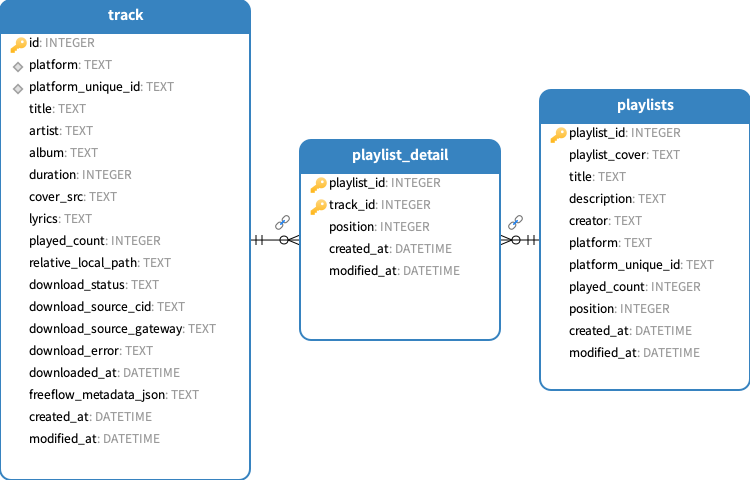
\includegraphics[width=0.95\textwidth]{figures/out/client_sqlite_er.png}
    \caption{客户端SQLite数据库ER图}
    \label{fig:client_sqlite_er}
\end{figure}

\begin{table}[htbp]
    \linespread{1.5}
    \zihao{5}
    \songti
    \centering
    \caption{客户端SQLite核心数据表说明}\label{tab:client_sqlite_tables}
    \begin{tabular}{|l|p{10cm}|}
        \hline
        数据表              & 设计说明                                                                \\ \hline
        track            & 保存统一歌曲记录，包括平台标识、平台内唯一ID、标题、歌手、专辑、封面、播放次数、本地文件路径、下载状态和FreeFlow链上扩展信息 \\ \hline
        playlists        & 保存用户歌单信息，包括标题、描述、封面、创建者、来源平台、播放次数和排序位置                              \\ \hline
        playlist\_detail & 保存歌单与歌曲的多对多关系，以playlist\_id和track\_id作为联合主键，并记录歌曲在歌单中的排序位置          \\ \hline
        sessions         & 保存应用启动会话，包括启动时间、操作系统和应用版本，用于记录桌面端运行情况                               \\ \hline
    \end{tabular}
\end{table}

\texttt{playlist\_detail}通过外键关联\texttt{playlists.playlist\_id}和\texttt{track.id}，删除歌单或歌曲时关联记录随之级联删除。音频下载模块会更新\texttt{track.relative\_local\_path}、\texttt{download\_status}、\texttt{download\_source\_cid}、\texttt{download\_source\_gateway}、\texttt{download\_error}和\texttt{downloaded\_at}等字段；链上音乐库则通过筛选\texttt{platform}为\texttt{FreeFlow}的\texttt{track}记录形成专门视图，无需另建一套重复的链上歌曲表。

\subsection{服务器PostgreSQL数据库设计}

服务器PostgreSQL数据库的核心ER关系如图\ref{fig:server_postgresql_er}所示。后端以\texttt{creator\_releases}作为链上音乐资源索引中心，围绕它关联创作者用户、IPFS存储对象、购买记录和评论记录。链上状态以智能合约为权威来源，后端数据库保存的是便于检索、展示和业务联动的链下投影。这样设计后，链上只承担权威状态确认，链下数据库则承担条件检索、分页展示、聚合统计和高频互动数据存储。

\begin{figure}[htbp]
    \centering
    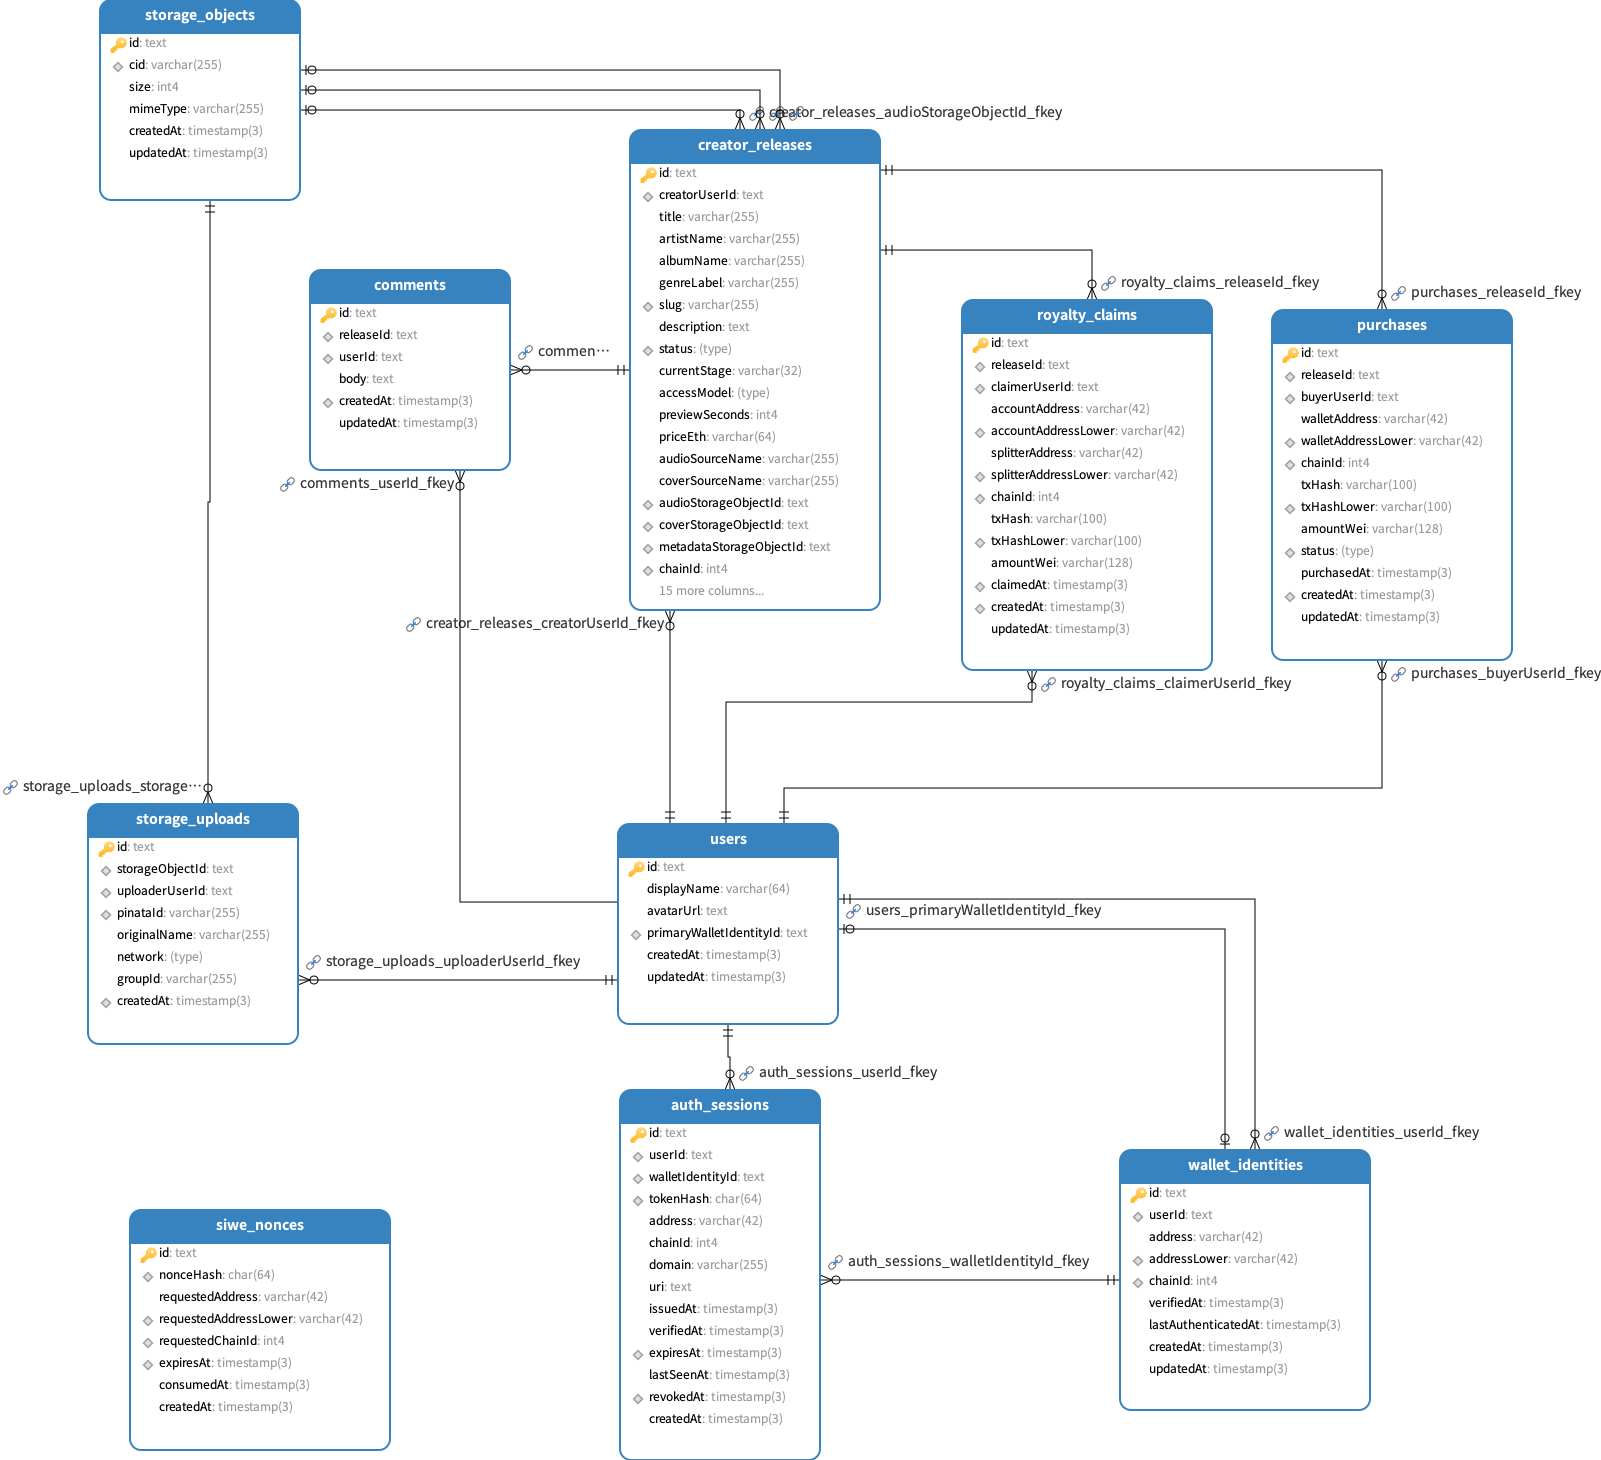
\includegraphics[width=0.98\textwidth]{figures/out/server_postgresql_er.png}
    \caption{服务器PostgreSQL数据库ER图}
    \label{fig:server_postgresql_er}
\end{figure}

\begin{table}[htbp]
    \linespread{1.5}
    \zihao{5}
    \songti
    \centering
    \caption{服务器PostgreSQL核心数据表说明}\label{tab:server_postgresql_tables}
    \begin{tabular}{|l|p{10cm}|}
        \hline
        数据表                & 设计说明                                                       \\ \hline
        users              & 保存系统用户资料，包含展示名、头像和主钱包身份引用                                  \\ \hline
        wallet\_identities & 保存钱包地址、链ID、验证时间和用户绑定关系，并通过addressLower与chainId保证同一链上地址唯一   \\ \hline
        siwe\_nonces       & 保存SIWE登录nonce哈希、请求地址、请求链ID、过期时间和消费时间，用于防止签名重放              \\ \hline
        auth\_sessions     & 保存登录会话token哈希、钱包身份、domain、uri、签发时间、验证时间、过期时间和吊销时间          \\ \hline
        storage\_objects   & 保存IPFS/Pinata对象的CID、文件大小和MIME类型，是音频、封面和metadata对象的统一记录     \\ \hline
        storage\_uploads   & 保存上传行为，关联上传者、存储对象、Pinata ID、原始文件名、存储网络和上传时间                \\ \hline
        creator\_releases  & 保存创作者发行项目和链上资源索引，包括作品元数据、发布阶段、访问模式、CID引用、合约地址、tokenId和交易哈希 \\ \hline
        purchases          & 保存购买交易投影，关联发行资源和购买用户，并用交易哈希、钱包地址、链ID等字段避免重复记录              \\ \hline
        comments           & 保存作品评论，关联发行资源和评论用户，并记录评论正文和时间信息                            \\ \hline
    \end{tabular}
\end{table}

\texttt{creator\_releases}表包含发行流程状态字段\texttt{status}和\texttt{currentStage}，用于支撑创作者工作台的阶段展示；包含\texttt{audioStorageObjectId}、\texttt{coverStorageObjectId}和\texttt{metadataStorageObjectId}，用于关联三类IPFS资源；包含\texttt{chainId}、\texttt{musicAssetAddress}、\texttt{platformHubAddress}、\texttt{splitterAddress}、\texttt{publishTxHash}、\texttt{publishBlockNumber}和\texttt{tokenId}，用于把链下发行记录定位到具体链上作品。系统对\texttt{chainId + musicAssetAddress + tokenId}设置唯一约束，确保同一链上访问凭证不会被重复索引。由此，资源搜索、详情页展示和排序计算都可以直接使用该链下索引，查询阶段也无需频繁遍历链上事件。

购买记录表\texttt{purchases}同时设置\texttt{chainId + txHashLower}和\texttt{releaseId + walletAddressLower + chainId}两组唯一约束。前者避免同一链上交易被重复写入，后者避免同一用户在同一链上对同一作品产生重复确认记录。评论表\texttt{comments}则以\texttt{releaseId}和\texttt{userId}分别建立索引，满足按作品拉取评论列表和按用户追踪评论行为的需求。评论数据保存在PostgreSQL中。评论需要频繁追加、分页读取、条件过滤和必要的内容处理，链下数据库更适合承载此类互动数据。


\section{智能合约设计}

系统合约由MusicAccess1155、PlatformHub和RoyaltySplitter组成。MusicAccess1155负责访问凭证，PlatformHub负责发布、购买和访问判断，RoyaltySplitter负责收益分账。

智能合约结构如图\ref{fig:contract_architecture}所示。创作者通过PlatformHub发布作品，PlatformHub在发布过程中调用RoyaltySplitterFactory为作品创建收益分账合约，并调用MusicAccess1155创建新的tokenId。听众购买付费作品时，PlatformHub校验销售配置和支付金额，随后调用MusicAccess1155铸造访问凭证，并将创作者及协作者对应的收益转入对应的RoyaltySplitter；平台手续费则保留在PlatformHub侧。这样的设计将平台收费与创作者侧分账分离，便于分别管理销售逻辑与收益提取逻辑。

\begin{figure}[htbp]
    \centering
    \includegraphics[width=0.95\textwidth]{figures/out/contract_architecture.png}
    \caption{智能合约结构图}
    \label{fig:contract_architecture}
\end{figure}

\begin{table}[htbp]
    \linespread{1.5}
    \zihao{5}
    \songti
    \centering
    \caption{智能合约职责说明}\label{tab:contract_design}
    \begin{tabular}{|l|p{10cm}|}
        \hline
        合约              & 职责                                    \\ \hline
        MusicAccess1155 & 为每首作品创建ERC-1155 tokenId，购买者持有不可转让访问凭证 \\ \hline
        PlatformHub     & 统一发布作品、保存销售配置、处理购买、判断访问状态和收取平台费       \\ \hline
        RoyaltySplitter & 按固定份额保存创作者和协作者收益，支持按地址提取              \\ \hline
    \end{tabular}
\end{table}


\section{系统安全设计}

系统安全设计主要包括以下方面：

\begin{enumerate}
    \item 身份认证安全：使用SIWE签名登录，后端校验nonce、地址、链ID、domain、uri和签发时间。
    \item 链上访问安全：付费作品的访问状态以ERC-1155凭证和合约hasAccess结果为依据。
    \item 交易安全：购买价格和销售状态由PlatformHub合约校验，避免客户端单独决定访问权。
    \item 接口安全：后端上传、发行、购买和评论等接口需要会话认证，并通过链下接口隔离高频业务写入与链上状态写入。
    \item 资源安全：当前IPFS资源仍存在CID公开后可直接访问的问题，后续可引入音频加密和授权网关。
\end{enumerate}



